\iffalse
\documentclass[journal,12pt,twocolumn]{IEEEtran}
%
\usepackage{setspace}
\usepackage{gensymb}
\usepackage{xcolor}
\usepackage{caption}
%\usepackage{subcaption}
%\doublespacing
\singlespacing
\usepackage{multicol}

\usepackage{iithtlc}
%\usepackage{graphicx}
%\usepackage{amssymb}
%\usepackage{relsize}
\usepackage[cmex10]{amsmath}
\usepackage{mathtools}
%\usepackage{amsthm}
%\interdisplaylinepenalty=2500
%\savesymbol{iint}
%\usepackage{txfonts}
%\restoresymbol{TXF}{iint}
%\usepackage{wasysym}
\usepackage{amsthm}
\usepackage{mathrsfs}
\usepackage{txfonts}
\usepackage{stfloats}
\usepackage{cite}
\usepackage{cases}
\usepackage{subfig}
%\usepackage{xtab}
\usepackage{longtable}
\usepackage{multirow}
%\usepackage{algorithm}
%\usepackage{algpseudocode}
\usepackage{enumitem}
\usepackage{mathtools}
%\usepackage{stmaryrd}

\usepackage{listings}
    \usepackage[latin1]{inputenc}                                 %%
    \usepackage{color}                                            %%
    \usepackage{array}                                            %%
    \usepackage{longtable}                                        %%
    \usepackage{calc}                                             %%
    \usepackage{multirow}                                         %%
    \usepackage{hhline}                                           %%
    \usepackage{ifthen}                                           %%
  %optionally (for landscape tables embedded in another document): %%
    \usepackage{lscape}     

%\usepackage{wasysym}
%\newcounter{MYtempeqncnt}
\DeclareMathOperator*{\Res}{Res}
%\renewcommand{\baselinestretch}{2}
\renewcommand\thesection{\arabic{section}}
\renewcommand\thesubsection{\thesection.\arabic{subsection}}
\renewcommand\thesubsubsection{\thesubsection.\arabic{subsubsection}}

\renewcommand\thesectiondis{\arabic{section}}
\renewcommand\thesubsectiondis{\thesectiondis.\arabic{subsection}}
\renewcommand\thesubsubsectiondis{\thesubsectiondis.\arabic{subsubsection}}

% correct bad hyphenation here
\hyphenation{op-tical net-works semi-conduc-tor}

\def\inputGnumericTable{}  

\lstset{
language=python,
frame=single, 
breaklines=true
}

\begin{document}
%

\theoremstyle{definition}

\newtheorem{theorem}{Theorem}[section]
\newtheorem{problem}{Problem}
\newtheorem{proposition}{Proposition}[section]
\newtheorem{lemma}{Lemma}[section]
\newtheorem{corollary}[theorem]{Corollary}
\newtheorem{example}{Example}[section]
\newtheorem{definition}{Definition}[section]
%\newtheorem{algorithm}{Algorithm}[section]
%\newtheorem{cor}{Corollary}
\newcommand{\BEQA}{\begin{eqnarray}}
\newcommand{\EEQA}{\end{eqnarray}}
\newcommand{\triangleq}{\stackrel{\triangle}{=}}

\bibliographystyle{IEEEtran}
%\bibliographystyle{ieeetr}



\providecommand{\pr}[1]{\ensuremath{\Pr\left(#1\right)}}
\providecommand{\qfunc}[1]{\ensuremath{Q\left(#1\right)}}
\providecommand{\sbrak}[1]{\ensuremath{{}\left[#1\right]}}
\providecommand{\lsbrak}[1]{\ensuremath{{}\left[#1\right.}}
\providecommand{\rsbrak}[1]{\ensuremath{{}\left.#1\right]}}
\providecommand{\brak}[1]{\ensuremath{\left(#1\right)}}
\providecommand{\lbrak}[1]{\ensuremath{\left(#1\right.}}
\providecommand{\rbrak}[1]{\ensuremath{\left.#1\right)}}
\providecommand{\cbrak}[1]{\ensuremath{\left\{#1\right\}}}
\providecommand{\lcbrak}[1]{\ensuremath{\left\{#1\right.}}
\providecommand{\rcbrak}[1]{\ensuremath{\left.#1\right\}}}
\theoremstyle{remark}
\newtheorem{rem}{Remark}
\newcommand{\sgn}{\mathop{\mathrm{sgn}}}
\providecommand{\abs}[1]{\left\vert#1\right\vert}
\providecommand{\res}[1]{\Res\displaylimits_{#1}} 
\providecommand{\norm}[1]{\lVert#1\rVert}
\providecommand{\mtx}[1]{\mathbf{#1}}
\providecommand{\mean}[1]{E\left[ #1 \right]}
\providecommand{\fourier}{\overset{\mathcal{F}}{ \rightleftharpoons}}
%\providecommand{\hilbert}{\overset{\mathcal{H}}{ \rightleftharpoons}}
\providecommand{\system}{\overset{\mathcal{H}}{ \longleftrightarrow}}
\providecommand{\gauss}[2]{\mathcal{N}\ensuremath{\left(#1,#2\right)}}
	%\newcommand{\solution}[2]{\textbf{Solution:}{#1}}
\newcommand{\solution}{\noindent \textbf{Solution: }}
\providecommand{\dec}[2]{\ensuremath{\overset{#1}{\underset{#2}{\gtrless}}}}
%\numberwithin{equation}{section}
%\numberwithin{problem}{section}

\def\putbox#1#2#3{\makebox[0in][l]{\makebox[#1][l]{}\raisebox{\baselineskip}[0in][0in]{\raisebox{#2}[0in][0in]{#3}}}}
     \def\rightbox#1{\makebox[0in][r]{#1}}
     \def\centbox#1{\makebox[0in]{#1}}
     \def\topbox#1{\raisebox{-\baselineskip}[0in][0in]{#1}}
     \def\midbox#1{\raisebox{-0.5\baselineskip}[0in][0in]{#1}}


% paper title
% can use linebreaks \\ within to get better formatting as desired
\title{
%\logo{
Digital Modulation Techniques
%}
}
%
%
% author names and IEEE memberships
% note positions of commas and nonbreaking spaces ( ~ ) LaTeX will not break
% a structure at a ~ so this keeps an author's name from being broken across
% two lines.
% use \thanks{} to gain access to the first footnote area
% a separate \thanks must be used for each paragraph as LaTeX2e's \thanks
% was not built to handle multiple paragraphs
%

%\author{Y Aditya, A Rathnakar and G V V Sharma$^{*}$% <-this % stops a space
\author{P.~N.~V.~S.~S.~K.~ HAVISH, S.~S.~Ashish and G V V Sharma %<-this  stops a space
\thanks{The authors are with the Department
of Electrical Engineering, IIT, Hyderabad
502285 India e-mail: \{ee16btech11023,ee16btech11043,jbala,gadepall\}@iith.ac.in. All material in the manuscript is released under GNU GPL.  Free to use for all.
}}



% make the title area
\maketitle

\tableofcontents

\bigskip

\begin{abstract}
%\boldmath
The manual frames the problems of receiver design and performance analysis in digital communication as applications of probability theory.

\end{abstract}
% IEEEtran.cls defaults to using nonbold math in the Abstract.
% This preserves the distinction between vectors and scalars. However,
% if the journal you are submitting to favors bold math in the abstract,
% then you can use LaTeX's standard command \boldmath at the very start
% of the abstract to achieve this. Many IEEE journals frown on math
% in the abstract anyway.

% Note that keywords are not normally used for peerreview papers.
%\begin{IEEEkeywords}
%Cooperative diversity, decode and forward, piecewise linear
%\end{IEEEkeywords}



% For peer review papers, you can put extra information on the cover
% page as needed:
% \ifCLASSOPTIONpeerreview
% \begin{center} \bfseries EDICS Category: 3-BBND \end{center}
% \fi
%
% For peerreview papers, this IEEEtran command inserts a page break and
% creates the second title. It will be ignored for other modes.
\IEEEpeerreviewmaketitle

\fi
\section{BPSK}
\begin{enumerate}
\item
The {\em signal constellation diagram} for BPSK is given by Fig. \ref{fig:bpsk_const}.  The symbols $s_0$ and $s_1$ are equiprobable.  $\sqrt{E_b}$ is the energy transmitted per bit. Assuming a zero mean additive white gaussian noise (AWGN) with variance $\frac{N_0}{2}$,
obtain the symbols that are received.

%
\begin{figure}[H]
\centering
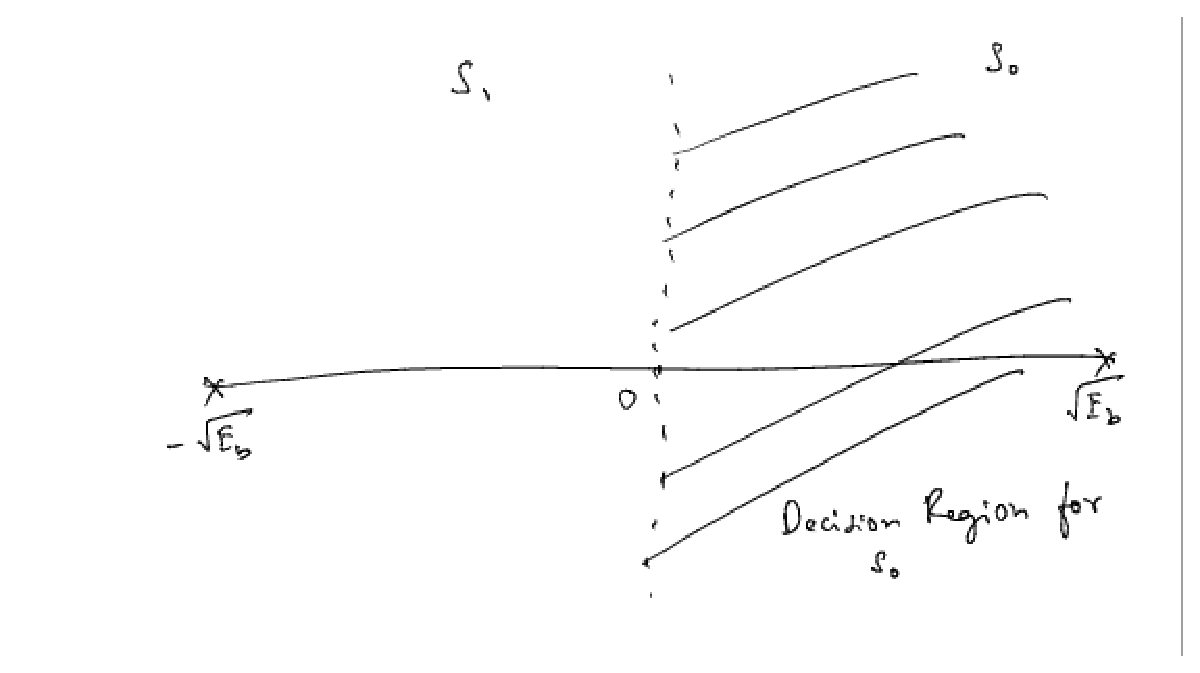
\includegraphics[width=\columnwidth]{./figs/bpsk_const.eps}
\caption{}
\label{fig:bpsk_const}
\end{figure}
\solution The possible received symbols are
\begin{align}
y|s_0 &= \sqrt{E_b} + n
\\
y|s_1 &= -\sqrt{E_b} + n
\end{align}
%
where the AWGN $n \sim \gauss{0}{\frac{N_0}{2}}$.
%
\item
\label{prob:bpsk_decision}
From Fig. \ref{fig:bpsk_const} obtain a decision rule for BPSK

\solution The decision rule is
\begin{equation}
y \dec{s_0}{s_1} 0
\end{equation}
\item
Repeat the previous exercise using the MAP criterion.\\
\solution When the symbols are equiprobable, the MAP rule stated in \eqref{eq:map_rule} simplifies to finding the symbol $s_i$ that %
maximizes the conditional PDF $p_Y(y|s_i)$ i.e.
\begin{align}
	\label{eq:mle_rule}
	\text{Set } \hat{x} &= x_i \text{ if}&\\ \nonumber
	p_Y(y|x_k) &\text{ is maximum for } k = i
\end{align}
In the case of BPSK, $y|s_0 \sim \gauss{\sqrt{E_b}}{\frac{N_0}{2}}$ and $y|s_1 \sim \gauss{-\sqrt{E_b}}{\frac{N_0}{2}}$. %
The two PDFs meet at $Y=0$. So,
\begin{align*}
	p_Y(y|s_0) > p_Y(y|s_1) &\text{ when } y > 0&\\
	p_Y(y|s_0) < p_Y(y|s_1) &\text{ when } y < 0 	
\end{align*}
The optimum threshold is therefore $Y=0$
\item
Using the decision rule in Problem \ref{prob:bpsk_decision}, obtain an expression for the probability of error for BPSK.
\solution
Since the symbols are equiprobable, it is sufficient if the error is calculated assuming that a 0 was sent.  This results in
\begin{align}
P_e &= \pr{y < 0|s_0} = \pr{\sqrt{E_b} + n < 0}
\\
&= \pr{ -n > \sqrt{E_b} } = \pr{ n > \sqrt{E_b} }
\label{eq:bpsk_proof_n0}
\end{align}
since $n$ has a symmetric pdf.
Let $w \sim \gauss{0}{1}$.  Then $n = \sqrt{\frac{N_0}{2}}w$. Substituting this in \eqref{eq:bpsk_proof_n0},
\begin{align}
P_e &=  \pr{ \sqrt{\frac{N_0}{2}}w > \sqrt{E_b} } = \pr{ w > \sqrt{\frac{2E_b}{N_0}} }
\\
&= \qfunc{\sqrt{\frac{2E_b}{N_0}}}
\end{align}
%
where $\qfunc{x} \triangleq \pr{w > x}, x \ge 0$.
\item
The PDF of $w \sim \gauss{0}{1}$ is given by
%
\begin{equation}
p_{w}(x) = \frac{1}{\sqrt{2\pi}}\exp\brak{-\frac{x^2}{2}}, -\infty < x < \infty
\end{equation}
and the complementary error function is defined as
\begin{equation}
\operatorname {erfc} (x)={\frac {2}{\sqrt {\pi }}}\int _{x}^{\infty }e^{-t^{2}}\,dt.
\end{equation}
%
Show that 
\begin{equation}
Q(x) = \frac{1}{2}\operatorname {erfc}\left({\frac  {x}{{\sqrt  {2}}}}\right)
\end{equation}\\
\solution From the definition of Q-function in \eqref{eq:q_func_integral},
\begin{align*}
	Q(x) &= \frac{1}{\sqrt{2\pi}}\int_{x}^{\infty} e^{-\frac{t}{2}} \,dt \\
	& \intertext{Substitute $u=\frac{t}{\sqrt{2}}$} \\
	Q(x) &= \frac{1}{\sqrt{\pi}}\int_{\frac{x}{\sqrt{2}}}^{\infty} e^{-u^2} \,du \\
	&= \frac{1}{2}\operatorname {erfc}\left({\frac  {x}{{\sqrt  {2}}}}\right)
\end{align*}

\item
Verify the bit error rate (BER) plots for BPSK through simulation and analysis for 0 to 10 dB.

\solution
The following code
%\lstinputlisting{./codes/bpsk_ber.py}
%\iffalse
\begin{lstlisting}
codes/chapter6/bpsk_ber.py
\end{lstlisting}
%	\fi
yields \ref{fig:bpsk_ber}
\begin{figure}[H]
\centering
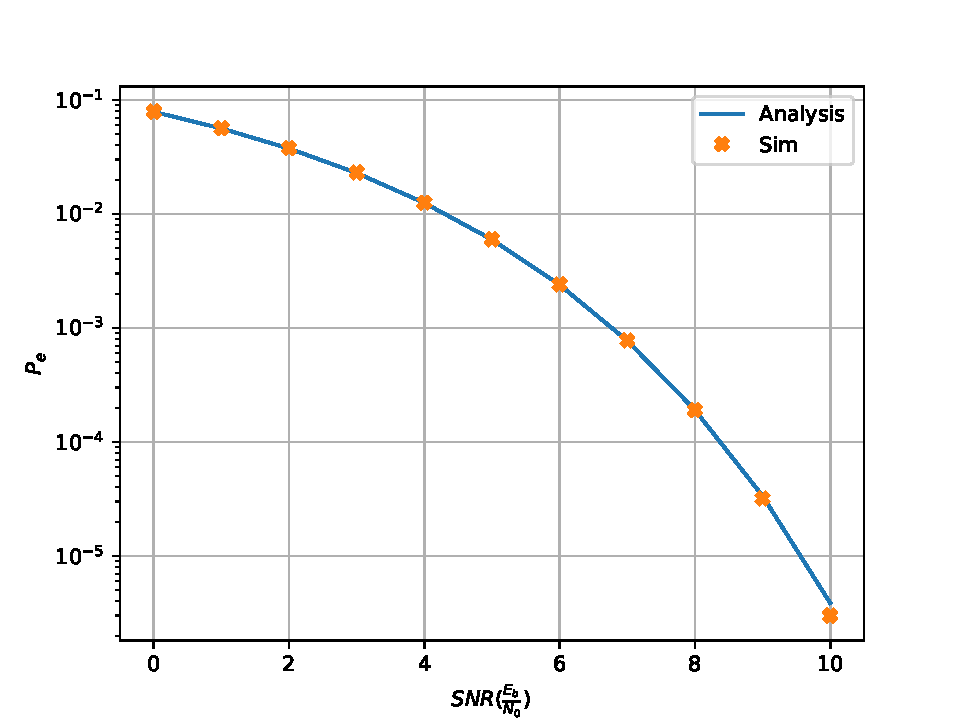
\includegraphics[width=\columnwidth]{./figs/bpsk_ber.pdf}
\caption{}
\label{fig:bpsk_ber}
\end{figure}

\item
\label{prob:craigs_formula_proof}
Show that
\begin{equation}
Q(x) = \frac{1}{\pi}\int^{\frac{\pi}{2}}_{0}e^{-\frac{x^2}{2\sin^2 \theta}}\,d\theta
\end{equation}\\
\solution Consider the bivariate gaussian distribution of $X,Y \sim \gauss{0}{1}$,
\begin{equation}
	p_{X,Y}(x,y) = \frac{1}{2\pi}\exp\left(-\frac{x^2+y^2}{2}\right)
	\label{eq:bivariate_std_gaussian_pdf}
\end{equation}
Using $p_{X,Y}(x,y)$, the Q-function can be expressed as,
\begin{align}
	Q(z) &= \int_{z}^{\infty}\int_{-\infty}^{\infty} p_{X,Y}(x,y) \,dx\,dy \\
	\label{eq:qfunc_biv_integ}
	&= \frac{1}{2\pi}\int_{z}^{\infty}\int_{-\infty}^{\infty} \exp\left(-\frac{x^2+y^2}{2}\right) \,dx\,dy
\end{align}
Transforming the integral in \eqref{eq:qfunc_biv_integ} to polar coordinates $(r,\theta)$ for $z > 0$,
\begin{align*}
	Q(z) &= \frac{1}{2\pi}\int_{-\frac{\pi}{2}}^{\frac{\pi}{2}}\int_{\frac{z}{\sin\theta}}^{\infty} \exp\left(-\frac{r^2}{2}\right)r \,dr\,d\theta\\
	&= \frac{1}{2\pi}\int_{-\frac{\pi}{2}}^{\frac{\pi}{2}} \exp\left(-\frac{z^2}{2\sin^2\theta}\right) \,d\theta\\
	&= \frac{1}{\pi}\int_{0}^{\frac{\pi}{2}} \exp\left(-\frac{z^2}{2\sin^2\theta}\right) \,d\theta \text{ , for $z > 0$}
\end{align*}
\end{enumerate}
\section{Coherent BFSK}
\begin{enumerate}
\item
The signal constellation for binary frequency shift keying (BFSK) is given in \ref{fig:bfsk_const}.
Obtain the equations for the received symbols.

\begin{figure}[H]
\centering
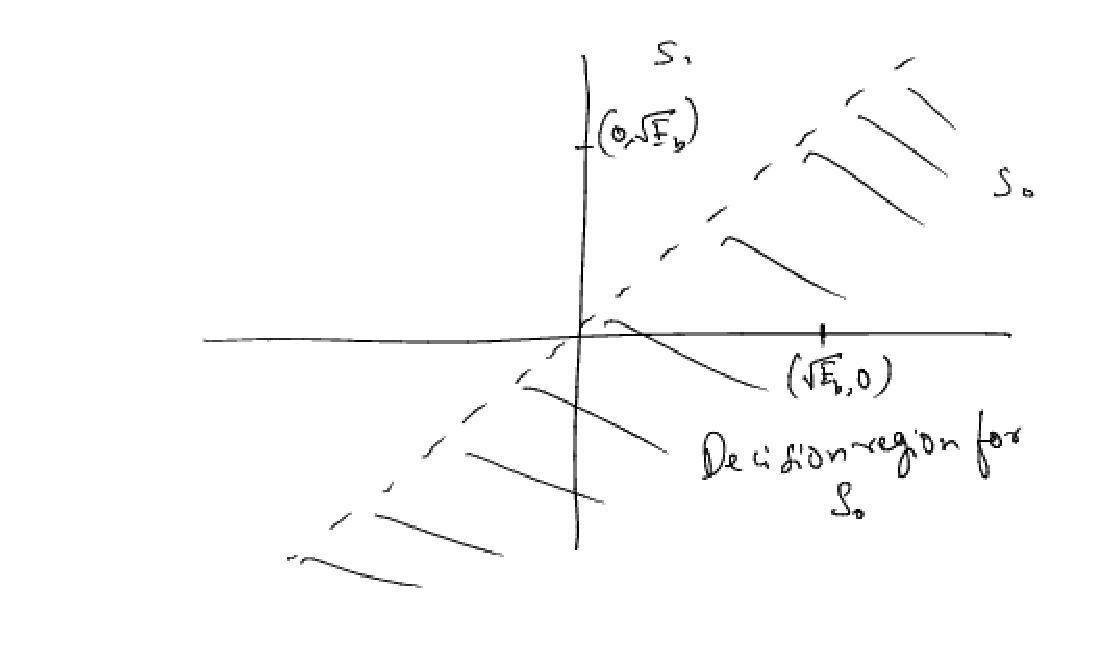
\includegraphics[width=\columnwidth]{./figs/bfsk_const.eps}
\caption{}
\label{fig:bfsk_const}
\end{figure}
\solution
The received symbols are given by
\begin{align}
\mathbf{y}|s_0 = 
\myvec{
\sqrt{E_b} \\
0
}
+
\myvec{
 n_{1}\\
n_{2}
},
\end{align}
and 
\begin{align}
\mathbf{y}|s_1 = 
\myvec{
0\\
\sqrt{E_b} 
}
+
\myvec{
n_{1}\\
 n_{2}
},
\end{align}
where $n_1,n_2 \sim \gauss{0}{\frac{N_0}{2}}$. and
$
\mathbf{y} = 
\myvec{
y_{1}\\
 y_{2}
}
$.
\item
Obtain a decision rule for BFSK from \ref{fig:bfsk_const}.

\solution The decision rule is
\begin{equation}
y_1 \dec{s_0}{s_1} y_2
\end{equation}
\item
Repeat the previous exercise using the MAP criterion.\\
\solution Let $\mbf{y} = \myvec{y_1&y_2&...&y_n}^T$ be the received signal. For an AWGN channel, given that symbol $\mbf{s_k}$ was sent, %
every component $y_i$ is normally distributed i.e. 
\begin{equation}
y_i|\mbf{s_k} \sim \gauss{s_{ki}}{\frac{N_0}{2}}\text{   ,} i=1,2,...,n 
\end{equation}
where $s_{ki}$ is the i$^{th}$ component of symbol $\mbf{s_k}$. Since all components of $\mbf{y}$ are independent, the joint PDF of $\mbf{y}$ given %
$\mbf{s_k}$ was sent is,
\begin{align}
	p_{\mbf{y}}(\mbf{y}|\mbf{s_k}) &= \prod\limits_{i=1}^{n} p_{y_i}(y_i|\mbf{s_k})&\\
	&= \left(\frac{2}{N_0\sqrt{2\pi}}\right)^n \exp\left(-\frac{2}{N_0^2}\sum\limits_{i=1}^{n} (y_i-s_{ki})^2\right)\\
	\label{eq:joint_pdf_fdistance}
	&= \left(\frac{2}{N_0\sqrt{2\pi}}\right)^n \exp\left(-\frac{2}{N_0^2}\norm{\vec{y}-\vec{s_k}}^2\right)
\end{align}
Ignoring the constants in \eqref{eq:joint_pdf_fdistance},
\begin{equation}
	p_{\mbf{y}}(\mbf{y}|\mbf{s_k}) \propto \exp\left(-\norm{\vec{y}-\vec{s_k}}^2\right)
\end{equation}
According to the MAP rule in \eqref{eq:mle_rule}, the optimal criterion to estimate $\vec{s}$ is to choose $\vec{\hat{s}}=\vec{s_k}$ whose
distance from $\vec{y}$ is minimum.
\begin{align}
	\label{eq:AWGN_est_rule}
	\text{Set } \hat{s} &= s_k \text{ if}&\\ \nonumber
	\norm{\vec{y}-\vec{s_i}}^2 & \text{ is minimum for } i = k
\end{align}
For the case of coherent BFSK, the locus for point equidistant from $\vec{s_0}$ and $\vec{s_1}$ is the line $y_1-y_2=0$. So, the optimum
decision is found as 
\begin{equation}
y_1 \dec{s_0}{s_1} y_2
\end{equation}

\item
Derive and plot the probability of error.  Verify through simulation.\\
\solution 
\begin{align}
	P_e &= \pr{y_1<y_2|s_0}\\
	&= \pr{\sqrt{E_b}+n_1<n_2}\\
	&= \pr{n_2-n_1 > \sqrt{E_b}}\\ \nonumber
	&= \pr{z > \sqrt{E_b}}, \text{where $z \sim \gauss{0}{N_0}$}\\
	&= \qfunc{\sqrt{\frac{E_b}{N_0}}}
\end{align}
The following code,
\begin{lstlisting}
codes/chapter6/bfsk_coherent_ber.py
\end{lstlisting}
yields \ref{fig:bfsk_coherent_ber}
\begin{figure}[H]
\centering
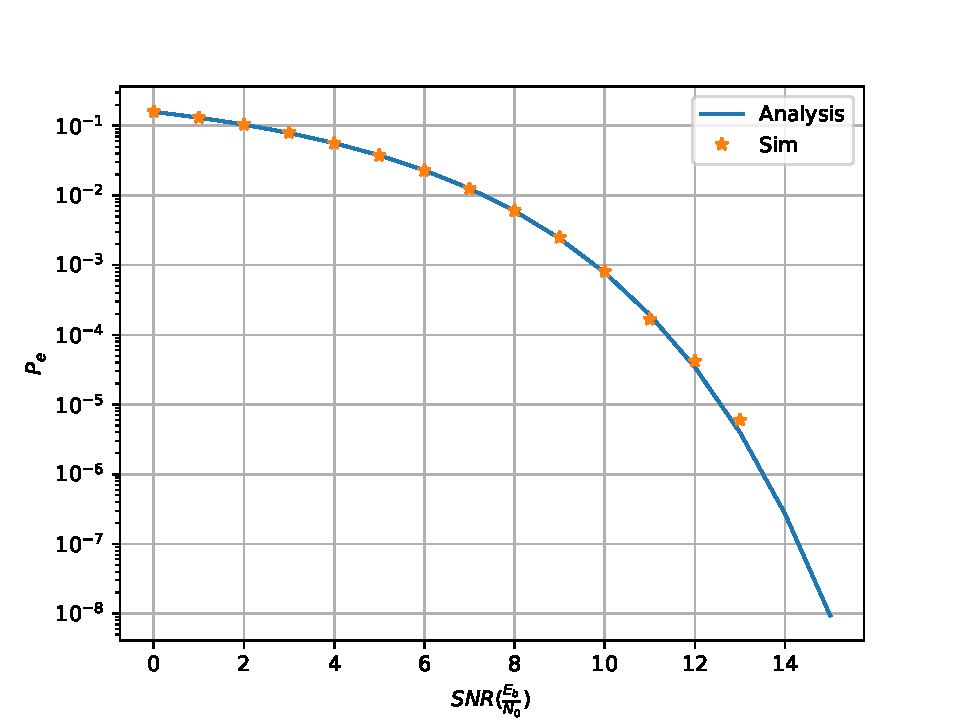
\includegraphics[width=\columnwidth]{./figs/bfsk_coherent_ber.pdf}
\caption{$P_e$ versus SNR for coherent BFSK}
\label{fig:bfsk_coherent_ber}
\end{figure}
\end{enumerate}

%
\section{QPSK}
\begin{enumerate}
\item
Let
\begin{equation}
\mathbf{r} = \mathbf{s}+ \mathbf{n}
\end{equation}
where $\mathbf{s} \in \cbrak{s_0,s_1,s_2, s_3}$ and
\begin{align}
\mathbf{s}_0 &= 
\myvec{
\sqrt{E_b}\\
0
},
\mathbf{s}_1 = 
\myvec{
0\\
\sqrt{E_b}
},
\\
\mathbf{s}_2 &= 
\myvec{
-\sqrt{E_b}\\
0
},
\mathbf{s}_3 = 
\myvec{
0\\
-\sqrt{E_b}
},
\\
E\sbrak{\mathbf{n}} &= \mathbf{0}, E\sbrak{\mathbf{n}\mathbf{n}^T} = \sigma^2 \mathbf{I}
\end{align}
%
\begin{enumerate}[label=(\alph{enumii})]
\item Show that the MAP decision for detecting $\mathbf{s}_0$ results in
\begin{equation}
\abs{r}_2 < r_1
\end{equation}\\
\solution For choosing $\vec{\hat{s}} = \vec{s_0}$, the below inequalities have to be satisfied (from \eqref{eq:AWGN_est_rule}).
\begin{align}
	\label{eq:qpsk_map_ineq1}
	\norm{\vec{r}-\vec{s_0}}^2 &< \norm{\vec{r}-\vec{s_1}}^2	\\
	\label{eq:qpsk_map_ineq2}
	\norm{\vec{r}-\vec{s_0}}^2 &< \norm{\vec{r}-\vec{s_2}}^2	\\
	\label{eq:qpsk_map_ineq3}
	\norm{\vec{r}-\vec{s_0}}^2 &< \norm{\vec{r}-\vec{s_3}}^2	
\end{align} 
Simplifying \eqref{eq:qpsk_map_ineq1},
\begin{align*}
	(\vec{r}-\vec{s_0})^{\top}(\vec{r}-\vec{s_0}) &< (\vec{r}-\vec{s_1})^{\top}(\vec{r}-\vec{s_1})\\
	\norm{r}^2 -2\vec{s_0}^{\top}\vec{r} + \norm{s_0}^2 &< \norm{r}^2 -2\vec{s_1}^{\top}\vec{r} + \norm{s_1}^2\\
	(\vec{s_1}-\vec{s_0})^{\top}\vec{r} &< 0 \text{\small,   $[\norm{s_0} = \norm{s_1} = \sqrt{E_b}$]}\\
	\myvec{-\sqrt{E_b}\\\sqrt{E_b}}^{\top}\vec{r} &< 0\\
	\myvec{-1\\1}^{\top}\vec{r} &< 0\\
	r_2 &< r_1
\end{align*}
Similarly, simplifying \eqref{eq:qpsk_map_ineq2} and \eqref{eq:qpsk_map_ineq3} we obtain
\begin{align*}
	r_2 &< r_1	\\
	-r_2 &< r_1 \\
	0 &< r_1	\\
	\implies \abs{r}_2 &< r_1
\end{align*} 

\item Express $\pr{\hat{\mathbf{s}} = \mathbf{s}_0|\mathbf{s} = \mathbf{s}_0}$ in terms of $r_1, r_2$.
Let $X=n_2-n_1, Y = -n_2-n_1$, where $\mathbf{n}=\brak{n_1,n_2}$.
Their correlation coefficient is defined as
%
\begin{align}
\rho = \frac{E\sbrak{\brak{X-\mu_x}\brak{Y-\mu_y}}}{\sigma_x\sigma_y}
\end{align}
%
$X$ and $Y$ are said to be uncorrelated if $\rho = 0$\\
\solution
\begin{flalign}
	\nonumber
	\pr{\hat{\mathbf{s}} = \mathbf{s}_0|\mathbf{s} = \mathbf{s}_0} &= \pr{\abs{r}_2 < r_1 | \mathbf{s} = \mathbf{s}_0}&\\
	\label{eq:qpsk_prob_error_r12}
	&= \pr{r_2 < r_1, -r_2 < r_1| \mathbf{s} = \mathbf{s}_0}
\end{flalign}
\
\item Show that if $X$ and $Y$ are uncorrelated 
Verify this numerically.\\
\solution Since $n_1$ and $n_2$ are independent,
\begin{align}
	p_{n_1,n_2}\brak{n_1,n_2} &= p_{n_1}\brak{n_1}p_{n_2}\brak{n_2}\\
	&= \frac{1}{2\pi\sigma} e^{-\frac{n_1^2+n_2^2}{2\sigma^2}}
\end{align}
Finding $\mu_x = E\sbrak{X}$,
\begin{align*}
	E\sbrak{X} &= E\sbrak{n_2-n_1}\\
	&= \int_{-\infty}^{\infty} \int_{-\infty}^{\infty} \brak{n_2-n_1}p_{n_1,n_2}\brak{n_1,n_2}  \,dn_1  \,dn_2\\
	&= \frac{1}{2\pi\sigma} \int_{-\infty}^{\infty} \int_{-\infty}^{\infty} \brak{n_2-n_1}e^{-\frac{n_1^2+n_2^2}{2\sigma^2}} \,dn_1  \,dn_2
\end{align*}
	
\begin{multline*}
	= \frac{1}{\sqrt{2\pi \sigma}}\left[ \int_{-\infty}^{\infty} e^{-\frac{n_2^2}{2\sigma^2}} \,dn_2 \right.\\
	\left. \frac{1}{\sqrt{2\pi \sigma}}\int_{-\infty}^{\infty} \brak{n_2-n_1} e^{-\frac{n_1^2}{2\sigma^2}} \,dn_1\right]
\end{multline*}
\begin{align*}
	&= \frac{1}{\sqrt{2\pi \sigma}} \int_{-\infty}^{\infty} n_2 e^{-\frac{n_2^2}{2\sigma^2}} \,dn_2\\
	&= 0
\end{align*} 
Similarly $\mu_y = 0$. Substituting $X, Y, \mu_x$ and $\mu_y$ in $\rho$,
\begin{align*}
	\rho &= \frac{E\sbrak{\brak{n_2-n_1}\brak{-n_2-n_1}}}{\sigma_X\sigma_Y}\\
	&= \frac{1}{\sigma_X \sigma_Y} \int_{-\infty}^{\infty} \int_{-\infty}^{\infty} \brak{n_1^2-n_2^2}p_{n_1,n_2}\brak{n_1,n_2}  \,dn_1  \,dn_2\\
	&= \frac{1}{\sigma_X \sigma_Y} \frac{1}{2\pi\sigma} \int_{-\infty}^{\infty} \int_{-\infty}^{\infty} \brak{n_1^2-n_2^2} e^{-\frac{n_1^2+n_2^2}{2\sigma^2}} \,dn_1  \,dn_2
\end{align*}
\begin{multline*}
	= \frac{1}{\sigma_X \sigma_Y} \frac{1}{\sqrt{2\pi \sigma}}\left[ \int_{-\infty}^{\infty} e^{-\frac{n_2^2}{2\sigma^2}} \,dn_2\right. \\
	\left. \frac{1}{\sqrt{2\pi \sigma}}\int_{-\infty}^{\infty} \brak{n_1^2-n_2^2} e^{-\frac{n_1^2}{2\sigma^2}} \,dn_1\right]
\end{multline*}
\begin{align*}
	&= \frac{1}{\sigma_x \sigma_y} \frac{1}{\sqrt{2\pi \sigma}} \int_{-\infty}^{\infty} \brak{\sigma^2-n_2^2} e^{-\frac{n_2^2}{2\sigma^2}} \,dn_2\\
	&= \frac{1}{\sigma_X \sigma_Y} \brak{\sigma^2-\sigma^2}\\
	&= 0
\end{align*}
The code below can be used to verify numerically that $\rho = 0$,
\begin{lstlisting}
codes/chapter6/zero_corr_verify.py
\end{lstlisting}
The output of the code is,
\begin{lstlisting}
Correlation coefficient is: 0.0002998	
\end{lstlisting}
The scatter plot in \ref{fig:zero_corr_scatter} visually shows that there is no significant correlation between $X$ and $Y$.
\begin{figure}[H]
\centering
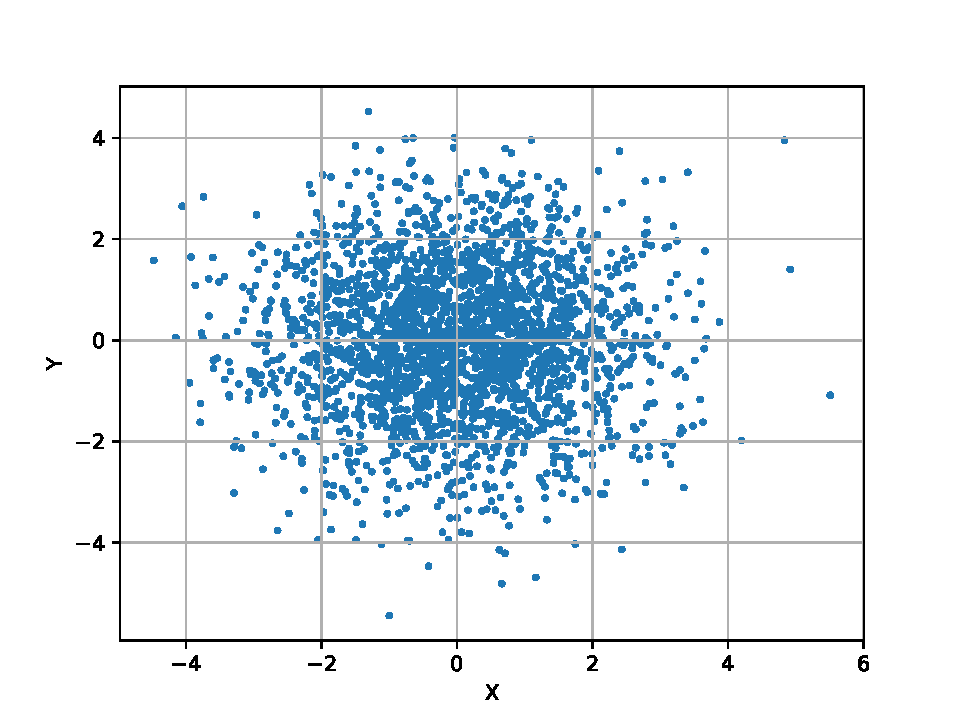
\includegraphics[width=\columnwidth]{./figs/zero_corr_verify.pdf}
\caption{Scatter plot of $X$ and $Y$}
\label{fig:zero_corr_scatter}
\end{figure}

\item Show that $X$ and $Y$ are independent, i.e. $p_{XY}(x,y) = p_{X}(x)p_{Y}(y)$.\\
\solution Since $X$ and $Y$ are linear combinations of Gaussian variables, $X$ and $Y$ are normally distributed. The joint PDF of two Gaussian %
variables is given by
\begin{multline}
	\label{eq:biv_gauss_gen}
	p_{X,Y}\brak{x,y} = \frac{1}{2\pi\sigma_X\sigma_Y\sqrt{1-\rho^2}}\\
	\exp\left\{-\frac{1}{2\brak{1-\rho^2}}\left[\brak{\frac{x-\mu_X}{\sigma_X}}^2+\brak{\frac{y-\mu_Y}{\sigma_Y}}^2\right.\right.\\
	\left.\left.-2\rho\frac{\brak{x-\mu_X}\brak{Y-\mu_Y}}{\sigma_X\sigma_Y}\right]\right\}
\end{multline}
Substituting $\rho = 0$,  
\begin{align}
	p_{X,Y}\brak{x,y} &= \frac{1}{2\pi\sigma_X\sigma_Y}\exp\cbrak{-\frac{\brak{x-\mu_X}^2}{2\sigma_X^2}-\frac{\brak{y-\mu_Y}^2}{2\sigma_Y^2}}\\
	&= \frac{1}{\sigma_X\sqrt{2\pi}}e^{-\frac{\brak{x-\mu_x}^2}{2\sigma_X^2}} \frac{1}{\sigma_Y\sqrt{2\pi}}e^{-\frac{\brak{y-\mu_y}^2}{2\sigma_Y^2}}\\
	&= p_X\brak{x} p_Y\brak{y}
\end{align}
\item Show that $X,Y \sim \mathcal{N}\brak{0,2\sigma^2}$.\\
\solution $X = n_2-n_1$ where $n_2, -n_1 \sim \gauss{0}{\sigma^2}$. The PDF of X is given by,
\begin{align}
	\nonumber
	p_X(x) &= p_{n_2}(n_2) \ast p_{-n_1}(n_1)\\\nonumber
	&= \frac{1}{2\pi\sigma^2}\int_{-\infty}^{\infty} e^{-\frac{t^2}{2\sigma^2}}e^{-\frac{(x-t)^2}{2\sigma^2}}  \,dt\\\nonumber
	&= \frac{1}{2\pi\sigma^2}\int_{-\infty}^{\infty} e^{-\frac{(x-t)^2+t^2}{2\sigma^2}}  \,dt\\\nonumber
	&= \frac{1}{2\pi\sigma^2}\int_{-\infty}^{\infty} e^{-\frac{(2t-x)^2+x^2}{2(\sqrt{2}\sigma)^2}}  \,dt\\\nonumber
	&= \frac{1}{2\pi\sigma^2}e^{-\frac{x^2}{2(\sqrt{2}\sigma)^2}}\int_{-\infty}^{\infty} e^{-\frac{(2t-x)^2}{2(\sqrt{2}\sigma)^2}}  \,dt\\\nonumber
	&= \frac{e^{-\frac{x^2}{2(\sqrt{2}\sigma)^2}}}{\sqrt{2\pi}\sqrt{2}\sigma} \frac{1}{\sqrt{2\pi}\sqrt{2}\sigma}\int_{-\infty}^{\infty} e^{-\frac{k^2}{2(\sqrt{2}\sigma)^2}}  \,dk\\
	\label{eq:std_gauss_diff_pdf}
	&= \frac{e^{-\frac{x^2}{2(\sqrt{2}\sigma)^2}}}{\sqrt{2\pi}\sqrt{2}\sigma}
\end{align}
From \eqref{eq:std_gauss_diff_pdf}, $X \sim \gauss{0}{2\sigma^2}$. Since $n_2$ and $-n_2$ are identically distributed (due to zero mean),
\begin{align*}
	p_Y(y) &= p_{-n_2}(n_2) \ast p_{-n_1}(n_1)\\
	&= p_{n_2}(n_2) \ast p_{-n_1}(n_1)\\
	&= p_X(x)
\end{align*}
So, $X,Y \sim \gauss{0}{2\sigma^2}$.
\item Show that $\pr{\hat{\mathbf{s}} = \mathbf{s}_0|\mathbf{s} = \mathbf{s}_0} =\pr{ X < A,  Y < A}$.\\
\solution From \eqref{eq:qpsk_prob_error_r12},
\begin{flalign*}
	\pr{\hat{\mathbf{s}} = \mathbf{s}_0| \mathbf{s} = \mathbf{s}_0} = \pr{r_2 < r_1, -r_2 < r_1 | \mathbf{s} = \mathbf{s}_0}&\\
	= \pr{n_2<n_1+\sqrt{E_b}, -n_2<n_1+\sqrt{E_b}}&\\
	= \pr{n_2-n_1<\sqrt{E_b}, -n_2-n_1<\sqrt{E_b}}&\\
	= \pr{X<\sqrt{E_b}, Y<\sqrt{E_b}}&\\
	= \pr{X<A, Y<A}
\end{flalign*}
\item Find $\pr{ X < A,  Y < A}$.\\
\solution Since $X$ and $Y$ are independant, 
\begin{flalign*}
	\pr{ X < A,  Y < A} = \pr{X<A}\pr{Y<A}
\end{flalign*}%
\begin{flalign*}
	&= F_X(A)F_Y(A)&\\
	&= \left(1-\qfunc{\frac{A}{\sqrt{2}\sigma}}\right)\left(1-\qfunc{\frac{A}{\sqrt{2}\sigma}}\right)&\\
	&= \left(1-\qfunc{\frac{A}{\sqrt{2}\sigma}}\right)^2&\\
	&= \left(1-\qfunc{\sqrt{\frac{E_b}{N_0}}}\right)^2 &\\
	& \text{since } A=\sqrt{E_b}, \sigma=\sqrt{\frac{N_0}{2}}&\\
	&= 1-2\qfunc{\sqrt{\frac{E_b}{N_0}}}+\qfunc{\sqrt{\frac{E_b}{N_0}}}^2&\\
	&\approx 1-2\qfunc{\sqrt{\frac{E_b}{N_0}}}&\\
	&= 1-\operatorname{erfc}\left(\sqrt{\frac{E_b}{2N_0}}\right)
\end{flalign*}
\item Verify the above through simulation.\\
\solution 
The following code,
\begin{lstlisting}
codes/chapter6/qfsk_ber.py
\end{lstlisting}
yields \ref{fig:qpsk_ber}. $P_e = 1-\pr{X<A,Y<A}$ plotted for SNR values from 0 to 10.
\begin{figure}[H]
\centering
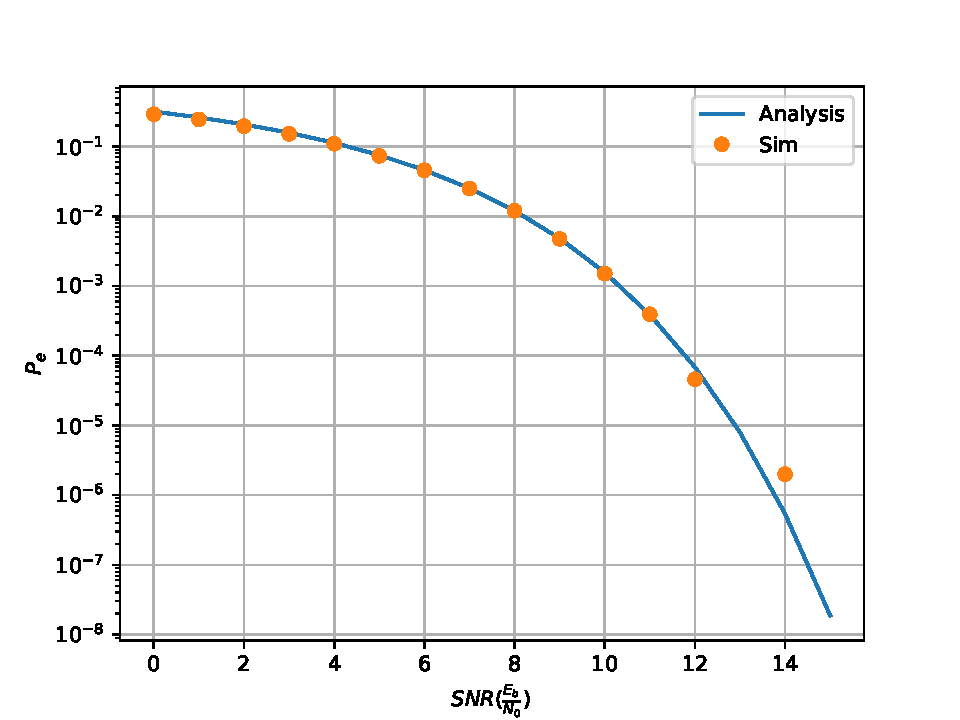
\includegraphics[width=\columnwidth]{./figs/qpsk_ber.pdf}
\caption{}
\label{fig:qpsk_ber}
\end{figure}
\end{enumerate}
\end{enumerate}

\section{$M$-PSK}
\begin{enumerate}

\item
Consider a system where 
$\mathbf{s}_i=
\myvec{
\cos\brak{\frac{2\pi i}{M}}\\
\sin\brak{\frac{2\pi i}{M}}
}, i = 0, 1 , \dots M-1
$
.
Let
%
\begin{align}
\mathbf{r}|s_0 = 
\myvec{
r_1\\
r_2
}
=
\myvec{
\sqrt{E_s}+n_1\\
n_2
}
\end{align}
where $n_1,n_2 \sim \mathcal{N}\brak{0,\frac{N_0}{2}}$.

\begin{enumerate}[label=(\alph{enumii})]
\item Substituting 
\label{prob:mpsk_polar_joint_pdf}
\begin{align}
r_1=R\cos \theta \\
r_2=R\sin \theta
\end{align}
show that the joint pdf of $R,\theta$ is
%
\begin{equation}
p\brak{R,\theta}=\frac{R}{\pi N_0}\exp\brak{-\frac{R^2-2R\sqrt{E_s}\cos \theta + E_s}{N_0}}
\label{eq:mpsk_joint_pdf_polar}
\end{equation}\\
\solution $r_1 \sim \gauss{\sqrt{E_s}}{\frac{N_0}{2}}$ and $r_2 \sim \gauss{0}{\frac{N_0}{2}}$. Since $r_1$ and $r_2$ are independent,
\begin{align*}
	p_{r_1,r_2}(r_1,r_2) &= p_{r_1}(r_1)p_{r_2}(r_2)
\end{align*}
\begin{align*}
	&= \frac{1}{\sqrt{\pi N_0}}\exp\left(-\frac{(r_1-\sqrt{E_s})^2}{N_0}\right)\frac{1}{\sqrt{\pi N_0}}\exp\left(-\frac{r_2^2}{N_0}\right)\\
	&= \frac{1}{\pi N_0}\exp\left(-\frac{(r_1-\sqrt{E_s})^2+r_2^2}{N_0}\right)
\end{align*}
Substituting for $r_1$ and $r_2$ in terms of $R$ and $\theta$
\begin{align*}
	p\brak{R,\theta} &= \frac{R}{\pi N_0}\exp\left(-\frac{(R\cos\theta - \sqrt{E_s})^2+R\sin^2\theta}{N_0}\right)\\
	&= \frac{R}{\pi N_0}\exp\brak{-\frac{R^2-2R\sqrt{E_s}\cos \theta + E_s}{N_0}}
\end{align*}
%
\item Show that 
%
\begin{align}
\label{eq:v_minus_alpha_integ}
\lim_{\alpha \rightarrow \infty}\int_{0}^{\infty}\brak{V-\alpha }e^{-\brak{V-\alpha}^2 }\,dV
&= 0
\\
\label{eq:no_v_minus_alpha_integ}
\lim_{\alpha \rightarrow \infty}\int_{0}^{\infty} e^{-\brak{V-\alpha}^2 }\,dV
&=  \sqrt{\pi}
\end{align}\\
\solution For \eqref{eq:v_minus_alpha_integ}, let $(V-\alpha)^2 = t$. Then
\begin{equation*}
	2(V-\alpha)dV = dt
\end{equation*} 
Changing the integral in terms of $t$,
\begin{align*}
	\lim_{\alpha \rightarrow \infty}\frac{1}{2}\int_{-\alpha^2}^{\infty}e^{-t}\,dt &= \lim_{\alpha \rightarrow \infty}\frac{1}{2}\sbrak{-e^{-t}}_{\alpha^2}^{\infty}\\
	&= \lim_{\alpha \rightarrow \infty}\frac{1}{2}e^{-\alpha^2}\\
	&= 0
\end{align*}
For \eqref{eq:no_v_minus_alpha_integ}, let $\brak{V-\alpha} = \frac{k}{\sqrt{2}}$. Then
\begin{equation*}
	dV = \frac{dk}{\sqrt{2}} 
\end{equation*} 
Changing the integral in terms of $k$,
\begin{align*}
	\lim_{\alpha \rightarrow \infty}\frac{1}{\sqrt{2}}\int_{-\sqrt{2}\alpha}^{\infty} e^{-\frac{k^2}{2}}\,dk &= \sqrt{\pi}\lim_{\alpha \rightarrow \infty}\frac{1}{\sqrt{2\pi}}\int_{-\sqrt{2}\alpha}^{\infty} e^{-\frac{k^2}{2}}\,dk\\
	&= \sqrt{\pi}\frac{1}{\sqrt{2\pi}}\int_{-\infty}^{\infty} e^{-\frac{k^2}{2}}\,dk\\
	&= \sqrt{\pi}
\end{align*}
%
\item 
Using the above, evaluate
%
\begin{align}
\int_{0}^{\infty}V\exp\cbrak{-\brak{V^2 - 2V \sqrt{\gamma}\cos \theta +\gamma}}\,dV
\end{align}
%
for large values of $\gamma$.\\
\solution By completing the square in the exponent, we get
\begin{align*}
	&\int_{0}^{\infty}Ve^{-\brak{(V - \sqrt{\gamma}\cos \theta)^2 +\gamma\sin^2 \theta}}\,dV\\
	&=e^{-\gamma\sin^2 \theta}\int_{0}^{\infty}Ve^{-\brak{V - \sqrt{\gamma}\cos \theta}^2}\,dV\\
	&=e^{-\gamma\sin^2 \theta}\left[\int_{0}^{\infty}\brak{V-\sqrt{\gamma}\cos \theta}e^{-\brak{V - \sqrt{\gamma}\cos \theta}^2}\right.\\
	&\left.+\sqrt{\gamma}\cos \theta \int_{0}^{\infty}e^{-\brak{V - \sqrt{\gamma}\cos \theta}^2}\,dV\right]
\end{align*}
Applying the limit $\gamma \rightarrow \infty$ and using the results from \eqref{eq:v_minus_alpha_integ} and \eqref{eq:no_v_minus_alpha_integ},
\begin{align}
	\nonumber
	&=\lim_{\gamma \rightarrow \infty}e^{-\gamma\sin^2 \theta}\int_{0}^{\infty}\brak{V-\sqrt{\gamma}\cos \theta}e^{-\brak{V - \sqrt{\gamma}\cos \theta}^2}\\
	\nonumber
	&+\lim_{\gamma \rightarrow \infty}e^{-\gamma\sin^2 \theta}\sqrt{\gamma}\cos \theta \int_{0}^{\infty}e^{-\brak{V - \sqrt{\gamma}\cos \theta}^2}\,dV\\
	\label{eq:limit_gamma_indet}
	&=0+\lim_{\gamma \rightarrow \infty}e^{-\gamma\sin^2 \theta}\sqrt{\gamma}\cos \theta \sqrt{\pi}
\end{align}
The value of \eqref{eq:limit_gamma_indet} is mainly determined by the product $e^{-\gamma\sin^2 \theta}\sqrt{\gamma}$ which has a $0\cdot\infty$ %
indeterminate form in the limit. Keeping the product without applying the limits,
\begin{equation}
	\int_{0}^{\infty}Ve^{-\brak{V^2 - 2V \sqrt{\gamma}\cos \theta +\gamma}}\,dV = e^{-\gamma\sin^2 \theta}\sqrt{\gamma\pi}\cos \theta
	\label{eq:v_integral_large_gamma}
\end{equation}
For large $\gamma$.
\item
Find a compact expression for 
%
\begin{align}
I = 1 - \sqrt{\frac{\gamma}{\pi}}\int_{-\frac{\pi}{M}}^{\frac{\pi}{M}}e^{- \gamma\sin^2\theta }\cos \theta\, d\theta
\end{align}\\
\solution Substituting $\sqrt{\gamma}\sin \theta=\frac{k}{\sqrt{2}}$,
\begin{align}
	\nonumber
	\sqrt{\gamma}\cos \theta d\theta &= \frac{dk}{\sqrt{2}}\\
	\nonumber
	\implies I &= 1 - \frac{1}{\sqrt{2\pi}}\int_{-\sqrt{2\gamma}\sin \frac{\pi}{M}}^{\sqrt{2\gamma}\sin \frac{\pi}{M}}e^{-\frac{k^2}{2}}\, dk\\
	\nonumber
	&= 1 - \left(1 - 2\qfunc{\sqrt{2\gamma}\sin \frac{\pi}{M}}\right)\\
	\label{eq:I_sector_Q_func}
	&= 2\qfunc{\sqrt{2\gamma}\sin \frac{\pi}{M}}\\
	&= \operatorname{erfc}\left(\sqrt{\gamma}\sin \frac{\pi}{M}\right)
\end{align}
\item Find $P_{e|\mathbf{s}_0}$.\\
\solution The optimal decision to detect $\vec{s}_0$ is,
\begin{align}
	\frac{\abs{r}_2}{\alpha} &< r_1\\
	\nonumber
	\text{where } \alpha &= \tan \frac{\pi}{M} 
\end{align}
$P_{e|\mathbf{s}_0}$ can then be found as 
\begin{align}
	P_{e|\mathbf{s}_0} &= 1 - \pr{\frac{\abs{r}_2}{\alpha} < r_1}
\end{align}
Appying the transformation from problem \ref{prob:mpsk_polar_joint_pdf} and using the joint pdf from \eqref{eq:mpsk_joint_pdf_polar},
\begin{align*}
	P_{e|\mathbf{s}_0} &= 1 - \pr{R < \infty, -\frac{\pi}{M} < \theta < \frac{\pi}{M}}\\
	&= 1 - \int_{-\frac{\pi}{M}}^{\frac{\pi}{M}} \int_{0}^{\infty} p\brak{R,\theta} \,dR  \,d\theta\\ 
	&= 1 - \frac{1}{\pi N_0} \int_{-\frac{\pi}{M}}^{\frac{\pi}{M}} \int_{0}^{\infty} Re^{-\frac{R^2-2R\sqrt{E_s}\cos \theta + E_s}{N_0}} \,dR  \,d\theta
\end{align*}
Substituting $V = \frac{R}{\sqrt{N_0}}$ and taking $\gamma = \frac{E_b}{N_0}$,
\begin{align*}
	P_{e|\mathbf{s}_0} &= 1 - \frac{1}{\pi} \int_{-\frac{\pi}{M}}^{\frac{\pi}{M}} \int_{0}^{\infty} Ve^{-\brak{V^2-2V\sqrt{\gamma}\cos \theta + \gamma}} \,dV  \,d\theta
\end{align*}
Using the result from \eqref{eq:v_integral_large_gamma},
\begin{align*}
	P_{e|\mathbf{s}_0} &= 1 - \frac{1}{\pi} \int_{-\frac{\pi}{M}}^{\frac{\pi}{M}}  e^{-\gamma\sin^2 \theta}\sqrt{\gamma\pi}\cos \theta \,d\theta\\
	&= 1 - \sqrt{\frac{\gamma}{\pi}} \int_{-\frac{\pi}{M}}^{\frac{\pi}{M}}  e^{-\gamma\sin^2 \theta}\cos \theta \,d\theta
\end{align*}
Using the result from \eqref{eq:I_sector_Q_func},
\begin{align}	
	P_{e|\mathbf{s}_0} &= 2\qfunc{\sqrt{2\gamma}\sin \frac{\pi}{M}}\\
	&= 2\qfunc{\sqrt{\frac{2E_b}{N_0}}\sin \frac{\pi}{M}}
\end{align}

\end{enumerate}
\end{enumerate}
\section{Noncoherent BFSK}
\begin{enumerate}
\item
Show that
%
\begin{align}
\label{eq:bessel_twopi}
I_{0}(x) &= \frac{1}{2\pi}\int_{0}^{2\pi}e^{x\cos\theta}\,d\theta \\
\label{eq:bessel_phi}
I_{0}(x) &= \frac{1}{2\pi}\int_{0}^{2\pi}e^{x\cos\brak{\theta-\phi}}\,d\theta \\
\label{eq:bessel_addition}
\frac{1}{2\pi}\int_{0}^{2\pi}e^{m_1\cos\theta + m_2\sin\theta}\,d\theta &= I_0\brak{\sqrt{m_1^2+m_2^2}} 
\end{align}
%
where the modified Bessel function of order $n$ (integer) is defined as 
%
\begin{align}
\label{eq:mod_bessel_n}
I_{n}(x) = \frac{1}{\pi}\int_{0}^{\pi}e^{x\cos\theta}\cos n\theta\,d\theta
\end{align}\\
\solution From \eqref{eq:mod_bessel_n}
\begin{equation}
	I_{0}(x) = \frac{1}{\pi}\int_{0}^{\pi}e^{x\cos\theta} \,d\theta
	\label{eq:mod_bessel_zero}
\end{equation}
Splitting the integral in \eqref{eq:bessel_twopi},
\begin{align}
	& \frac{1}{2\pi}\left[\int_{0}^{\pi}e^{x\cos\theta}\,d\theta+\int_{\pi}^{2\pi}e^{x\cos\theta}\,d\theta\right]\\
	\label{eq:bessel_twopi_inter}
	& \frac{1}{2\pi}\left[\pi I_{0}(x)+\int_{0}^{\pi}e^{-x\cos\theta}\,d\theta\right]
\end{align}
Since $-\cos \theta$ is monotonic and lies between $[-1,1]$ for $\theta \in [0,\pi]$, $e^{x\cos\theta}$ and $e^{-x\cos\theta}$ are symmetric %
for $\theta \in [0,\pi]$ about $\theta = \frac{\pi}{2}$. So,
\begin{align}
	\label{eq:bessel_twopi_eq_integ}
	\int_{0}^{\pi}e^{x\cos\theta}\,d\theta = \int_{0}^{\pi}e^{-x\cos\theta}\,d\theta
\end{align}
Substituting \eqref{eq:bessel_twopi_eq_integ} in \eqref{eq:bessel_twopi_inter},
\begin{align*}
	& \frac{1}{2\pi}\left[\pi I_{0}(x)+\int_{0}^{\pi}e^{x\cos\theta}\,d\theta\right]\\
	&= \frac{1}{2\pi}\left[\pi I_{0}(x)+\pi I_{0}(x)\right]\\
	&= I_{0}(x)
\end{align*}
Substituting $\theta-\phi = \omega$ in \eqref{eq:bessel_phi},
\begin{align}
	\label{eq:bessel_phi_inter}
	I_{0}(x) &= \frac{1}{2\pi}\int_{-\phi}^{2\pi-\phi}e^{x\cos\brak{\omega}}\,d\omega
\end{align}
Since $\cos \omega$ is periodic with period $2\pi$,
\begin{equation}
	\int_{0}^{2\pi} \cos \omega \,d\omega = \int_{\alpha}^{2\pi+\alpha} \cos \omega \,d\omega
	\label{eq:periodic_integral}
\end{equation}
Using \eqref{eq:periodic_integral} in \eqref{eq:bessel_phi_inter},
\begin{align*}
	& \frac{1}{2\pi}\int_{0}^{2\pi}e^{x\cos\brak{\omega}}\,d\omega\\
	&= I_{0}(x) &\text{ from \eqref{eq:bessel_twopi}}
\end{align*}
Using the trigonomentric identity,
\begin{align}
	\label{eq:trig_identity_ab}
	m_1\cos\theta + m_2\sin\theta &= \sqrt{m_1^2+m_2^2}\cos\brak{\theta-\phi}\\
	\nonumber
	\text{where } \tan \phi &= \frac{m_2}{m_1} 
\end{align}
the integral in \eqref{eq:bessel_addition} is given by,
\begin{align*}
	&\frac{1}{2\pi}\int_{0}^{2\pi}e^{\sqrt{m_1^2+m_2^2}\cos\brak{\theta-\phi}}\,d\theta \\
	&= I_{0}\brak{\sqrt{m_1^2+m_2^2}} &\text{from \eqref{eq:bessel_phi}} 
\end{align*}
\item
Let
%
\begin{align}
\mathbf{r}|0= \sqrt{E_b}
\myvec{
\cos \phi_0\\
\sin \phi_0 \\
0\\
0
}
+\mathbf{n}_0,
\mathbf{r}|1= \sqrt{E_b}
\myvec{
0\\
0 \\
\cos \phi_1\\
\sin \phi_1 
}
+\mathbf{n}_1
\end{align}
%
where $\mathbf{n}_0,\mathbf{n}_1\sim \mathcal{N}\brak{\mathbf{0}, \frac{N_0}{2}\mathbf{I}}$.
%
\begin{enumerate}[label=(\alph{enumii})]
\item Taking $\mathbf{r} = \brak{r_1,r_2,r_3,r_4}^{T},$, find the pdf $p\brak{\mathbf{r}|0,\phi_0}$ in
terms of $r_1,r_2,r_3,r_4,\phi,E_b$ and $N_0$. Assume that all noise variables are independent.\\
\solution Since $r_1, r_2, r_3, r_4$ are independant,
\begin{equation}
	p\brak{\mathbf{r}|0,\phi_0} = \prod_{i=1}^{4} p\brak{r_i|0,\phi_0}
	\label{eq:product_pdf_noncoh_bfsk}
\end{equation}
Substituting the PDFs for 
\begin{equation}
\vec{r}|0,\phi_0 \sim \gauss{\sqrt{E_b}\myvec{\cos \phi_0\\\sin \phi_0\\0\\0}}{\frac{N_0}{2}\vec{I}}
\end{equation}
in \eqref{eq:product_pdf_noncoh_bfsk}, we get
\begin{align}
	\nonumber
	p\brak{\mathbf{r}|0,\phi_0}&\\
	=\frac{1}{N_0^2\pi^2}&e^{-\frac{\brak{r_1-\sqrt{E_b}\cos \phi_0}^2+\brak{r_2-\sqrt{E_b}\sin \phi_0}^2+r_3^2+r_4^2}{N_0}}
\end{align}
%
\item 
If $\phi_0$ is uniformly distributed between 0 and $2\pi$, find $p\brak{\mathbf{r}|0}$.  Note that this expression will no longer contain $\phi_0$.\\
\solution
\begin{flalign*}
	p\brak{\mathbf{r}|0} &= \int_{0}^{2\pi} p\brak{\mathbf{r}|0,\phi_0} \,d\phi_0
\end{flalign*}
\begin{flalign*}
	=\frac{1}{N_0^2\pi^2}\int_{0}^{2\pi}e^{-\frac{\brak{r_1-\sqrt{E_b}\cos \phi_0}^2+\brak{r_2-\sqrt{E_b}\sin \phi_0}^2+r_3^2+r_4^2}{N_0}} \,d\phi_0\\
	=\frac{1}{N_0^2\pi^2}e^{-\frac{r_1^2+r_2^2+r_3^2+r_4^2+E_b}{N_0}}\int_{0}^{2\pi}e^{\frac{2\sqrt{E_b}}{N_0}\brak{r_1\cos \phi_0 + r_2\sin \phi_0}} \,d\phi_0
\end{flalign*}
\begin{flalign}
	\label{eq:noncoh_bfsk_pdf}
	=\frac{1}{N_0^2\pi^2}e^{-\frac{r_1^2+r_2^2+r_3^2+r_4^2+E_b}{N_0}}I_{0}\brak{\frac{2\sqrt{E_b}}{N_0}\sqrt{r_1^2+r_2^2}}&\\
	\nonumber
	\text{from \eqref{eq:bessel_addition}}&
\end{flalign}
%
\item
Show that the ML detection criterion for this scheme is
%
\begin{align}
\label{eq:noncoh_bfsk_decision_comp}
I_0\brak{k\sqrt{r_1^2+r_2^2}}\dec{0}{1}I_0\brak{k\sqrt{r_3^2+r_4^2}}
\end{align}
%
where $k$ is a constant.\\
\solution The PDF of $\vec{r}|1$ has a similar form to \eqref{eq:noncoh_bfsk_pdf},
\begin{equation}
	p\brak{\mathbf{r}|1} = \frac{1}{N_0^2\pi^2}e^{-\frac{r_1^2+r_2^2+r_3^2+r_4^2+E_b}{N_0}}I_{0}\brak{\frac{2\sqrt{E_b}}{N_0}\sqrt{r_3^2+r_4^2}}
	\label{eq:noncoh_bfsk_pdf_one}
\end{equation}
From \eqref{eq:noncoh_bfsk_pdf} and \eqref{eq:noncoh_bfsk_pdf_one},
\begin{align}
	p\brak{\mathbf{r}|0} &=  f(\vec{r}) I_{0}\brak{k\sqrt{r_1^2+r_2^2}}\\
	p\brak{\mathbf{r}|1} &=  f(\vec{r}) I_{0}\brak{k\sqrt{r_3^2+r_4^2}}
\end{align}
Using the MLE rule from \eqref{eq:mle_rule}, the optimum decision is given by
\begin{align}
I_0\brak{k\sqrt{r_1^2+r_2^2}}\dec{0}{1}I_0\brak{k\sqrt{r_3^2+r_4^2}}
\end{align}
%
\item 
The above criterion reduces to something simpler.  Can you guess what it is?  Justify your answer.\\
\solution Since $I_{0}(x)$ is monotonic for $x \ge 0$, and since the arguements to the Bessel function in \eqref{eq:noncoh_bfsk_decision_comp} %
are positive, the decision simplifies to
\begin{align}
	\nonumber
	\sqrt{r_1^2+r_2^2}\dec{0}{1}\sqrt{r_3^2+r_4^2}\\
	\label{eq:noncoh_bfsk_decision_simp}
	\implies \brak{r_1^2+r_2^2}\dec{0}{1}\brak{r_3^2+r_4^2}
\end{align}
%
\item 
Show that 
%
\begin{align}
P_{e|0}=\pr{r_1^2+r_2^2 < r_3^2+r_4^2 | 0}
\end{align}\\
\solution From \eqref{eq:noncoh_bfsk_decision_simp},
\begin{align}
P_{e|0} &= \pr{\hat{\vec{s}} = \vec{s}_1 | \vec{s} = \vec{s}_0}\\
	&=\pr{r_1^2+r_2^2 < r_3^2+r_4^2 | 0}
\end{align}
%
\item 
Show that the pdf of $Y=r_3^2+r_4^2$ id
%
\begin{align}
\label{eq:noncoh_bfsk_r34sq_pdf}
p_{Y}(y) = \frac{1}{N_0}e^{-\frac{y}{N_0}}, y > 0
\end{align}\\
\solution Using \eqref{eq:square_pdf_gen}, the PDF of $Z=r_3^2$ is given by
\begin{align}
	\nonumber
	p_Z(z) &= \frac{1}{2\sqrt{z}}p_{r_1}\brak{\sqrt{z}} + p_{r_1}\brak{-\sqrt{z}}\\
	\nonumber
	&= \frac{1}{2\sqrt{\pi N_0 z}}\brak{e^{-\frac{r_1}{N_0}}+e^{-\frac{r_1}{N_0}}}\\
	\label{eq:bfsk_r34sq_pdf}
	&= \frac{1}{\sqrt{\pi N_0 z}}e^{-\frac{r_1}{N_0}}
\end{align}
Since $r_3$ and $r_4$ are identically distributed, $r_4^2$ has the same PDF as $Z$. Since $Y$ is the sum of two independant random variables,
\begin{flalign*}
	p_Y(y) &= p_{r_3^2}(r_3) \ast p_{r_4^2}(r_4)&\\
	&= \frac{1}{\pi N_0} \int_{0}^{y} \frac{e^{-\frac{x}{N_0}}}{\sqrt{x}}\frac{e^{-\frac{y-x}{N_0}}}{\sqrt{y-x}}  \,dx&\\
	&= \frac{e^{-\frac{y}{N_0}}}{\pi N_0} \int_{0}^{y} \frac{1}{\sqrt{x(y-x)}}  \,dx&\\
	&= \frac{e^{-\frac{y}{N_0}}}{\pi N_0} \sbrak{-\arcsin\left(\dfrac{y-2x}{v}\right)}_0^v&\\
	&= \frac{e^{-\frac{y}{N_0}}}{\pi N_0} \pi&\\
	&= \frac{e^{-\frac{y}{N_0}}}{N_0} \text{ for } y \ge 0
\end{flalign*}
%
\item 
Find 
%
\begin{align}
g\brak{r_1,r_2} = \pr{r_1^2+r_2^2<Y|0,r_1,r_2}.
\end{align}\\
\solution Using the PDF of $Y$ from \eqref{eq:noncoh_bfsk_r34sq_pdf},
\begin{align}
	\pr{r_1^2+r_2^2<Y|0,r_1,r_2} &= \int_{r_1^2+r_2^2}^{\infty} \frac{e^{-\frac{y}{N_0}}}{N_0}  \,dy\\
	&= \sbrak{-e^{-\frac{y}{N_0}}}_{r_1^2+r_2^2}^{\infty}\\
	&= e^{-\frac{r_1^2+r_2^2}{N_0}}
\end{align}
\item 
Show that $E\sbrak{e^{-\frac{X^2}{2\sigma^2}}}=\frac{1}{\sqrt{2}}e^{-\frac{\mu^2}{4\sigma^2}}$ for $X \sim 
\mathcal{N}\brak{\mu,\sigma^2}$.\\
\solution 
\begin{align}
	\nonumber
	E\sbrak{e^{-\frac{X^2}{2\sigma^2}}} &= \frac{1}{\sigma \sqrt{2\pi}} \int_{-\infty}^{\infty} e^{-\frac{x^2}{2\sigma^2}}e^{-\frac{(x-\mu)^2}{2\sigma^2}}  \,dx\\\nonumber
	&= \frac{1}{\sigma \sqrt{2\pi}}\int_{-\infty}^{\infty} e^{-\frac{(x-\mu)^2+x^2}{2\sigma^2}}  \,dx\\\nonumber
	&= \frac{1}{\sigma \sqrt{2\pi}}\int_{-\infty}^{\infty} e^{-\frac{(2x-\mu)^2+\mu^2}{2(\sqrt{2}\sigma)^2}}  \,dx\\\nonumber
	&= e^{-\frac{\mu^2}{4\sigma^2}}\frac{1}{\sigma \sqrt{2\pi}}\int_{-\infty}^{\infty} e^{-\frac{(2x-\mu)^2}{2(\sqrt{2}\sigma)^2}}  \,dx\\\nonumber
	&= \frac{e^{-\frac{\mu^2}{4\sigma^2}}}{\sqrt{2}}\frac{1}{\sqrt{2}\sigma \sqrt{2\pi}}\int_{-\infty}^{\infty} e^{-\frac{k^2}{2(\sqrt{2}\sigma)^2}}  \,dk\\
	\label{eq:noncoh_bfsk_expg}
	E\sbrak{e^{-\frac{X^2}{2\sigma^2}}} &= \frac{1}{\sqrt{2}}e^{-\frac{\mu^2}{4\sigma^2}}
\end{align}
%
\item 
Now show that
%
\begin{align}
E\sbrak{g\brak{r_1,r_2}}=\frac{1}{2}e^{-\frac{E_b}{2N_0}}.
\end{align}\\
\solution Since $r_1$ and $r_2$ are independent,
\begin{multline*}
E\sbrak{g\brak{r_1,r_2}} =\\ 
\int_{-\infty}^{\infty} \int_{-\infty}^{\infty} g\brak{r_1,r_2} p_{r_1}\brak{r_1} p_{r_2}\brak{r_2} \,dr_1  \,dr_2
\end{multline*}
\begin{flalign}
\nonumber
= \int_{-\infty}^{\infty} \int_{-\infty}^{\infty} e^{-\frac{r_1^2+r_2^2}{N_0}} p_{r_1}\brak{r_1} p_{r_2}\brak{r_2} \,dr_1  \,dr_2 &\\
\label{eq:noncoh_bfsk_exp_integ_prod}
= \int_{-\infty}^{\infty} e^{-\frac{r_1^2}{N_0}} p_{r_1}\brak{r_1} \,dr_1 \int_{-\infty}^{\infty} e^{-\frac{r_2^2}{N_0}} p_{r_2}\brak{r_2} \,dr_2
\end{flalign}
Since $r_1,r_2 \sim \gauss{\sqrt{E_b}\myvec{\cos \phi_0 & \sin \phi_0}^{\top}}{\frac{N_0}{2}\vec{I}}$, \eqref{eq:noncoh_bfsk_expg} can be used %
to evaluate the integrals in \eqref{eq:noncoh_bfsk_exp_integ_prod},
\begin{align}
	E\sbrak{g\brak{r_1,r_2}} &= \frac{1}{\sqrt{2}}e^{-\frac{E_b \cos^2 \phi_0}{2 N_0}} \frac{1}{\sqrt{2}}e^{-\frac{E_b \sin^2 \phi_0}{2 N_0}}\\
	&= \frac{1}{2}e^{\frac{E_b \brak{\cos^2 \phi_0 + \sin^2 \phi_0}}{2 N_0}}\\
	&=\frac{1}{2}e^{-\frac{E_b}{2N_0}}
\end{align}
%
\end{enumerate}
\item
 Let $U,V\sim\mathcal{N}\brak{0,\frac{k}{2}}$ be i.i.d.  Assuming that
%
\begin{align}
U = \sqrt{R} \cos \Theta \\
V = \sqrt{R} \sin \Theta
\end{align}
\begin{enumerate}[label=(\alph{enumii})]
\item 
Compute the jacobian for $U,V$ with respect to $X$ and $\Theta$ defined by
%
\begin{align}
J = \det\brak{
\begin{matrix}
\frac{\partial U}{\partial R} & \frac{\partial U}{\partial \Theta} \\
\frac{\partial V}{\partial R} & \frac{\partial V}{\partial \Theta}
\end{matrix}
}
\end{align}\\
\solution 
\begin{align}
J = \det\brak{
\begin{matrix}
\frac{\cos \Theta}{2\sqrt{R}} & -\sqrt{R}\sin \Theta \\
\frac{\sin \Theta}{2\sqrt{R}} & \sqrt{R}\cos \Theta
\end{matrix}
}\\
= \frac{1}{2}\brak{\cos^2\Theta + \sin^2\Theta}&\\
= \frac{1}{2}&
\end{align}
\item 
The joint pdf for $R,\Theta$ is given by,
%
\begin{align}
p_{R,\Theta}\brak{r,\theta} = p_{U,V}\brak{u,v}J\vert_{u = \sqrt{r}\cos\theta,v = \sqrt{r}\sin\theta}
\end{align}
Show that
%
\begin{align}
p_{R}(r) = 
\begin{cases}
\frac{1}{k}e^{-\frac{r}{k}} & r > 0, \\
0 & r < 0,
\end{cases}
\end{align}
%
assuming that $\Theta$ is uniformly distributed between 0 to $2\pi$.\\
\solution Since $U,V\sim\mathcal{N}\brak{0,\frac{k}{2}}$ are i.i.d,
\begin{align}
	p_{U,V}\brak{u,v} &= \frac{1}{k\pi}e^{-\frac{u^2+v^2}{k}}
\end{align}
Transforming from $(U,V)$ to $(R,\Theta)$,
\begin{align}
	p_{R,\Theta}\brak{r,\theta} &= \frac{J}{k\pi}e^{-\frac{r\cos^2\Theta+r\sin^2\Theta}{k}}\\
	&= \frac{1}{2k\pi}e^{-\frac{r}{k}} \text{ for $r > 0$}
\end{align}
Finding marginal PDF w.r.t $R$,
\begin{align}
	p_{R}\brak{r} &= \int_{0}^{2\pi} p_{R,\Theta}\brak{r,\theta} \,d\Theta\\
	&= \frac{1}{k2\pi}e^{-\frac{r}{k}} \int_{0}^{2\pi} \,d\Theta\\
	&= \frac{1}{k}e^{-\frac{r}{k}} \text{ for $r > 0$}
\end{align}
\begin{equation}
	p_{R}\brak{r} = 
	\begin{cases}
		\frac{1}{k} e^{-\frac{r}{k}} & r > 0\\
		0 & r < 0
	\end{cases}
	\label{eq:noncoh_bfsk_pdf_y}
\end{equation}
%
\item
Show that the pdf of $Y = R_1-R_2$, where $R_1$ and $R_2$ are i.i.d. and have the same distribution as $R$ is
%
\begin{align}
p_{Y}(y) = \frac{1}{2k}e^{-\frac{\abs{y}}{k}}
\end{align}\\
\solution Given the PDF of $Y$ is given by
\begin{align}
	p_{Y}\brak{y} &= p_{R_1}\brak{r_1} \ast p_{R_2}\brak{-r_2}\\
	&=
	\begin{cases}
		\int_{0}^{\infty} p_{R_1}\brak{t} p_{R_2}\brak{t-y}  \,dt & y < 0\\
		\int_{y}^{\infty} p_{R_1}\brak{t} p_{R_2}\brak{t-y}  \,dt & y > 0
	\end{cases}
\end{align}
Evaluating the integral for $y < 0$,
\begin{align}
	\int_{0}^{\infty} p_{R_1}\brak{t} p_{R_2}\brak{t-y}  \,dt &= \frac{1}{k^2} \int_{0}^{\infty} e^{-\frac{t}{k}}e^{-\frac{t-y}{k}} \,dt\\
	&= \frac{e^{\frac{y}{k}}}{k^2} \int_{0}^{\infty} e^{-\frac{2t}{k}} \,dt\\
	\label{eq:indefenite_convolution_y_bfsk}
	&= \frac{e^{\frac{y}{k}}}{k^2} \sbrak{-\frac{k}{2}e^{-\frac{2t}{k}}}_{0}^{\infty}\\
	\label{eq:noncoh_bfsk_conv_y_p1}
	&= \frac{1}{2k}e^{\frac{y}{k}} \text{ , for $y < 0$}
\end{align}
Substituting limits of the integral for $y > 0$ in \eqref{eq:indefenite_convolution_y_bfsk},
\begin{align}
	&= \frac{e^{\frac{y}{k}}}{k^2} \sbrak{-\frac{k}{2}e^{-\frac{2t}{k}}}_{y}^{\infty}\\
	&= \frac{e^{\frac{y}{k}}}{k^2} \frac{k}{2}e^{-\frac{2y}{k}}\\
	\label{eq:noncoh_bfsk_conv_y_p2}
	&= \frac{1}{2k}e^{\frac{-y}{k}} \text{ , for $y > 0$}
\end{align}
Combining \eqref{eq:noncoh_bfsk_conv_y_p1} and \eqref{eq:noncoh_bfsk_conv_y_p2},
\begin{align}
p_{Y}(y) = \frac{1}{2k}e^{-\frac{\abs{y}}{k}}
\end{align}
%
\item 
 Find the pdf of 
%
\begin{align}
Z = p + \sqrt{p}\sbrak{U \cos \phi + V \sin \phi}
\end{align}
%
where $\phi$ is a constant.\\
\solution Let $A = \brak{\sqrt{p}\cos \phi} U$ and $B = \brak{\sqrt{p}\sin \phi} V$. Then,
\begin{align}
	A \sim \gauss{0}{\frac{kp \cos^2\phi}{2}}\\
	B \sim \gauss{0}{\frac{kp \sin^2\phi}{2}}
\end{align} 
If $C=A+B$, then
\begin{align}
	C \sim \gauss{0}{\frac{kp}{2}}
\end{align}
Since $Z=p+C$, $Z \sim \gauss{p}{\frac{kp}{2}}$. The PDF of $Z$ is given by,
\begin{align}
	p_{Z}\brak{z} = \frac{1}{\sqrt{kp\pi}}e^{-\frac{\brak{z-p}^2}{kp}}
\end{align}
\item 
Find $\pr{Y > Z}$.\\
Let $g\brak{z} = \pr{Y > z|Z = z}$. Evaluating $g\brak{z}$,
\begin{align}
	\pr{Y > z|Z = z} = \int_{z}^{\infty} p_Y\brak{y} \,dy\\
	= \int_{z}^{\infty} \frac{1}{2k}e^{-\frac{\abs{y}}{k}} \,dy\\
	=
	\begin{cases}
		\int_{z}^{\infty} \frac{1}{2k}e^{-\frac{y}{k}} \,dy & z > 0\\
		\int_{z}^{0} \frac{1}{2k}e^{\frac{y}{k}} \,dy + \int_{0}^{\infty} \frac{1}{2k}e^{-\frac{y}{k}}\,dy & z < 0
	\end{cases}\\
	g\brak{z} =
	\begin{cases}
		\frac{1}{2}e^{-\frac{z}{k}} & z > 0\\
		1-\frac{1}{2}e^{\frac{z}{k}}  & z < 0
	\end{cases}
\end{align}
$\pr{Y > Z}$ is calculated as $E\sbrak{g\brak{z}}$,
\begin{align}
	&E\sbrak{g\brak{z}} = \int_{-\infty}^{\infty} g\brak{z}p_{Z}\brak{z} \,dz\\
	\label{eq:noncoh_bfsk_exp_z_int}
	&=  \int_{-\infty}^{0} \brak{1-\frac{1}{2}e^{\frac{z}{k}}} p_Z\brak{z} \,dz +  \int_{0}^{\infty} \frac{1}{2}e^{-\frac{z}{k}}p_Z\brak{z} \,dz\\
	&= I_1 + I_2
\end{align}
Substituting $p_Z\brak{z}$ in $I_1$,
\begin{align}
	I_1 &= \int_{-\infty}^{0} \brak{1-\frac{1}{2}e^{\frac{z}{k}}} \frac{1}{\sqrt{kp\pi}}e^{-\frac{\brak{z-p}^2}{kp}} \,dz\\
	&= \frac{1}{\sqrt{kp\pi}}\brak{\int_{-\infty}^{0} e^{-\frac{\brak{z-p}^2}{kp}} \,dz - \int_{-\infty}^{0} \frac{1}{2}e^{\frac{z}{k}} e^{-\frac{\brak{z-p}^2}{kp}}} \,dz
\end{align}
Substituting $t = \frac{z}{\sqrt{kp}}$ and $\gamma = \frac{p}{k}$,
\begin{multline}
	I_1 = \frac{1}{\sqrt{\pi}}\left(\int_{-\infty}^{0} e^{-\brak{t-\sqrt{\gamma}}^2} \,dt \right.\\
	\left. - \frac{1}{2} \int_{-\infty}^{0} e^{t \sqrt{\gamma}} e^{-\brak{t-\sqrt{\gamma}}^2} \,dt \right)
\end{multline}
\begin{align}
	&= \frac{1}{\sqrt{\pi}}\int_{-\infty}^{0} e^{-\brak{t-\sqrt{\gamma}}^2} \,dt - \frac{e^{\frac{5\gamma}{4}}}{2\sqrt{\pi}} \int_{-\infty}^{0} e^{-\brak{t-\frac{\sqrt{3\gamma}}{2}}^2} \,dt
\end{align}
Since area under a Gaussian curve is unity, from \eqref{eq:no_v_minus_alpha_integ} it can concluded that,
\begin{align}
	\label{eq:no_v_minus_alpha_integ_comp}
	\lim_{\alpha \rightarrow \infty} \int_{-\infty}^{0} e^{-\brak{V-\alpha}^2} \,dV = 0
\end{align}
Let $\sqrt{\gamma} = \alpha$. Computing $I_1$ for large values of $\alpha$,
\begin{multline}
	\lim_{\alpha \rightarrow \infty} I_1 = \lim_{\alpha \rightarrow \infty} \frac{1}{\sqrt{\pi}} \int_{-\infty}^{0} e^{-\brak{t-\alpha}^2} \,dt\\
	- \lim_{\alpha \rightarrow \infty} \frac{e^{\frac{5\alpha^2}{4}}}{2\sqrt{\pi}} \int_{-\infty}^{0} e^{-\brak{t-\frac{3\alpha}{2}}^2} \,dt
\end{multline}
Using \eqref{eq:no_v_minus_alpha_integ_comp},
\begin{align}
	\lim_{\alpha \rightarrow \infty} I_1 &= 0 - \lim_{\alpha \rightarrow \infty} \frac{e^{\frac{5\alpha^2}{4}}}{2\sqrt{\pi}} \int_{-\infty}^{0} e^{-\brak{t-\frac{3\alpha}{2}}^2} \,dt\\
	&= -\frac{1}{2\sqrt{\pi}} \lim_{\alpha \rightarrow \infty} \frac{\int_{-\infty}^{0} e^{-\brak{t-\frac{3\alpha}{2}}^2 \,dt}}{e^{-\frac{5\alpha^2}{4}}}
\end{align}
Using L'Hopital's rule,
\begin{align}
	\lim_{\alpha \rightarrow \infty} I_1 &= \frac{1}{2\sqrt{\pi}} \lim_{\alpha \rightarrow \infty} \frac{6}{5} \frac{\int_{-\infty}^{0} \brak{t-\frac{3\alpha}{2}} e^{-\brak{t-\frac{3\alpha}{2}}^2} \,dt}{\alpha e^{-\frac{5\alpha^2}{4}}}
\end{align}
\item 
If $U\sim\mathcal{N}\brak{m_1,\frac{k}{2}},V\sim\mathcal{N}\brak{m_2,\frac{k}{2}}$, where $m_1,m_2, k$ are constants, show that the pdf of 
%
\begin{align}
R = \sqrt{U^2+V^2}
\end{align}
%
is
%
\begin{align}
\label{eq:general_chi_sq}
p_{R}\brak{r} = \frac{e^{-\frac{r +m}{k}}}{ k}I_{0}\brak{\frac{2\sqrt{mr}}{k}},\quad m = \sqrt{m_1^2+m_2^2}
\end{align}\\
\solution The CDF of $R$ is given by.
\begin{align}
	F_{R}\brak{r} &= \pr{R < r} \text{ , for $r > 0$}\\
	&= \pr{\sqrt{U^2 + V^2} < r}\\
	&= \pr{U^2 + V^2 < r^2}
\end{align}
The area of integration to obtain $F_{R}\brak{r}$ is the circle with radius $r$.
\begin{align}
	F_{R}\brak{r} &= \int_{-r}^{r} \int_{-\sqrt{r^2-v^2}}^{\sqrt{r^2-v^2}} p_{U,V}\brak{u,v}  \,du  \,dv\\
	&= \int_{-r}^{r} \int_{-\sqrt{r^2-v^2}}^{\sqrt{r^2-v^2}} p_{U}\brak{u} p_{V}\brak{v} \,du  \,dv\\
	\nonumber
	&\text{   \small (since $U$ and $V$ are independent)}\\
	&= \int_{-r}^{r} \int_{-\sqrt{r^2-v^2}}^{\sqrt{r^2-v^2}} \frac{1}{k\pi} e^{-\frac{\brak{u-m_1}^2+\brak{v-m_2}^2}{k}} \,du  \,dv
\end{align}
Transforming the integral to polar coordinates with $u=R \cos \theta$ and $v=R \sin \theta$,
\begin{align}
	F_{R}\brak{r} &= \frac{1}{k\pi} \int_{0}^{r} \int_{0}^{2\pi} Re^{-\frac{\brak{R\cos \theta-m_1}^+\brak{R\sin \theta-m_2}^2}{k}} \,dR  \,d\theta  
\end{align}
To find $p_{R}\brak{r}$, differentiate $F_{R}\brak{r}$ w.r.t $r$ using Leibniz's rule.
\begin{align}
	p_{R}\brak{r} &= \frac{1}{k\pi} \int_{0}^{2\pi} re^{-\frac{\brak{r\cos \theta-m_1}^2+\brak{r\sin \theta-m_2}^2}{k}} \,d\theta\\ 
	&= \frac{1}{k\pi}re^{-\frac{r^2+m_1^2+m_2^2}{k}} \int_{0}^{2\pi} e^{\frac{2r m_1}{k}\cos \theta + \frac{2r m_2}{k}\sin \theta} \,d\theta
\end{align}
Using \eqref{eq:bessel_addition},
\begin{align}
	p_{R}\brak{r} &= \frac{2}{k}re^{-\frac{r^2+m_1^2+m_2^2}{k}}I_{0}\brak{\frac{2r}{k}\sqrt{m_1^2+m_2^2}}\\
	&= \frac{2}{k}re^{-\frac{r^2+m^2}{k}}I_{0}\brak{\frac{2rm}{k}} \text{, $m=\sqrt{m_1^2+m_2^2}$}
\end{align}
%
\item
Show that
\begin{align}
I_0(x) = \sum_{n=0}^{\infty}\frac{x^{2n}}{4^n\brak{n!}^2}
\end{align}\\
\solution The modified bessel function of first kind is given by
\begin{align}
	\label{eq:mod_bessel_eq_series}
	I_{n}\brak{x} = \brak{\frac{1}{2}x}^n \sum_{k=0}^{\infty} \frac{\brak{\frac{1}{4}x^2}^k}{k!\Gamma\brak{n+k+1}}
\end{align}
Substituting $n=0$,
\begin{align}
	I_{0}\brak{x} &= \sum_{k=0}^{\infty} \frac{\brak{\frac{1}{4}x^2}^k}{k!\Gamma\brak{k+1}}\\
	&= \sum_{k=0}^{\infty} \frac{x^{2k}}{4^k\brak{k!}^2}
\end{align}
\item 
If
%
\begin{align}
p_{Z}(z) &= 
\begin{cases}
\frac{1}{k} e^{-\frac{z}{k}} & z \geq 0 \\
0 & z < 0
\end{cases}
\end{align}
%
find $\pr{R < Z}$.
\end{enumerate}
\end{enumerate}
\section{Craig's Formula and MGF}
\begin{enumerate}
\item
The Moment Generating Function (MGF) of $X$ is defined as
%
\begin{align}
M_{X}(s) = E\sbrak{e^{s X}}
\end{align}
%
where $X$ is a random variable and $E\sbrak{\cdot}$ is the expectation.  
%
%
\begin{enumerate}[label=(\alph{enumii})]
\item Let $Y \sim \gauss{0}{1}$.  Define
%
\begin{align}
Q(x) = \pr{Y > x}, x > 0
\end{align}
%
Show that
\begin{equation}
Q(x) = \frac{1}{\pi}\int^{\frac{\pi}{2}}_{0}e^{-\frac{x^2}{2\sin^2 \theta}}\,d\theta
\end{equation}
\solution Refer solution to problem \ref{prob:craigs_formula_proof}.
\item 
Let $h\sim\mathcal{CN}\brak{0,\frac{\Omega}{2}},n\sim\mathcal{CN}\brak{0,\frac{N_0}{2}}$.  Find the distribution of $\abs{h}^2$.\\
\solution $\abs{h}^2 = \Re\cbrak{h}^2 + \Im\cbrak{h}^2$ where $\Re\cbrak{h}, \Im\cbrak{h} \sim \gauss{0}{\frac{\Omega}{4}}$. Let $R=\abs{h}^2$. %
Using \eqref{eq:general_chi_sq}, $p_R\brak{r}$ is given by
\begin{align}
	p_{R}\brak{r} &= \frac{2}{\Omega}e^{-\frac{2r}{\Omega}}
\end{align}
\item Let
%
\begin{align}
P_e = \pr{\Re \cbrak{h^*y} < 0}, \text{ where } y = \brak{\sqrt{E_s}h + n},
\end{align}
%
Show that
%
\begin{align}
P_e = \int_{0}^{\infty}\qfunc{\sqrt{2x}}p_{A}(x) \,dx
\end{align}
where $A = \frac{E_s\abs{h}^2}{N_0}$.
\item Show that
%
\begin{align}
P_e 
%&= E\sbrak{\qfunc{\sqrt{2A}}} \\
%&=  \frac{1}{\pi}\int_{0}^{\frac{\pi}{2}}E\sbrak{e^{-\frac{A}{\sin^2\theta}}}\,d\theta \\
&=  \frac{1}{\pi}\int_{0}^{\frac{\pi}{2}}M_{A}\brak{-\frac{1}{\sin^2\theta}}\,d\theta
\label{ch4_pe_mgf}
\end{align}
%
\item compute $M_A(s)$.
%
\item 
Find $P_e$.
\item 
If $\gamma = \frac{\Omega E_s}{N_0}$, show that $P_e < \frac{1}{2\gamma}$. 
\end{enumerate}
\end{enumerate}
%
\fi
